\documentclass{beamer}

\usepackage{array}
\usepackage[english]{babel}
\usepackage[utf8x]{inputenc}
\usepackage{amssymb}
\usepackage{amsmath}
\usepackage{geometry}
\usepackage{graphicx}
\usepackage{eucal}
\usepackage{cite}
\usepackage{wrapfig}
\usepackage{datetime}
\usepackage[font=small,labelfont=bf]{caption}

\graphicspath{ {./fig} }
\setbeamertemplate{bibliography item}{\insertbiblabel}

\title{Public key cryptography + concept of secure messaging}
\author{Alexander Buchnev}

\newdateformat{monthYear}{\monthname[\THEMONTH] \THEYEAR}
\date{\monthYear\today}

\DeclareCaptionFormat{custom}
{%
    \textbf{\tiny #1#2}\textit{\tiny #3}
}
\captionsetup{format=custom}

\begin{document}

\frame{
	\titlepage
}

\newtheorem{prop}{Proposition}

%% Proof for the homework

\begin{frame}{Outline}
    \section{Outline}
	\tableofcontents
\end{frame}

\begin{frame}{New directions in cryptography}
    \section{New directions in cryptography}
    In their groundbreaking article \cite{diffie-hellman:1976}, Diffie and Hellman propose new concepts and techniques
    of secure messaging that are still in use (article dates back to 1976!!).
\end{frame}

\begin{frame}{A method for obtaining digital signatures and public-key cryptosystems}
    \section{A method for obtaining digital signatures and public-key cryptosystems}
    A year later, Ronald Rivest, Adi Shamir and Leonard Adleman publish a paper \cite{rsa-1978}, which describes the algorithm, that
	later received name ``RSA''. The proposed method for obtaining public-key cryptosystems is based on underlying problem of integer
    factorisation. 
\end{frame}

\begin{frame}{A method for obtaining digital signatures and public-key cryptosystems}
    For now, there is no evidence that the RSA cryptosystem is prone to polynomial-time attacks running on classical
    computers, although there are many problems one could face constructing secure 
    implementation of the RSA PKC (we will talk about that in a couple of lectures).
\end{frame}

\begin{frame}{Perfect secrecy}
	\section{Perfect secrecy}
    \begin{wrapfigure}{R}{0.5\textwidth}
        \begin{center}
        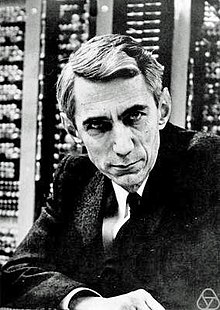
\includegraphics[height=0.35\textheight]{shannon.jpg}
        \end{center}
    \caption{Claude Shannon \\ (source: \href{https://wikipedia.org}{wikipedia.org})}
    \end{wrapfigure}
    In 1948, Claude Shannon published the article `A Mathematical Theory of Communication' \cite{shannon-1948}, where he introduces the notion of entropy as a measure
    of information content in a message. The higher the entropy, the higher the uncertainty of the next symbol in the message and vice
    versa.
\end{frame}

\begin{frame}{Entropy}
    \subsection{Entropy}
    As it was said earlier, entropy (or uncertainty) is the measure of the information content. 
    Claude Shannon defines entropy in the following way:
\end{frame}

\begin{frame}{Entropy}
    \begin{definition}[Entropy]
        Suppose we have a set of possible events whose probabilities of occurence are
        $(p_1, p_2, \ldots, p_n)$. We want to derive an entropy measure $H$ on 
        these probabilities. \\
        ``If there is such measure $H$, it is reasonable to require of it the 
        following properties:''
        \begin{enumerate}
            % entropy.pdf pages 10-11
            \item $H$ should be continuous on $p_i$
            \item If all $p_i$ are equal to $p_i = \frac{1}{n}$, then $H$ should
            be a monotonic increasing function of $n$. With equally likely events
            there is more choice, thus more uncertainty.
        \end{enumerate} 
    \end{definition}
\end{frame}

\begin{frame}{Entropy cnt.}
    \begin{definition}[Entropy cnt.]
        \begin{enumerate}
            \setcounter{enumi}{2}
            \item  If a choice be broken down into two successive choices, the 
            original $H$ should be the weighted sum of the individual values of $H$.
            
            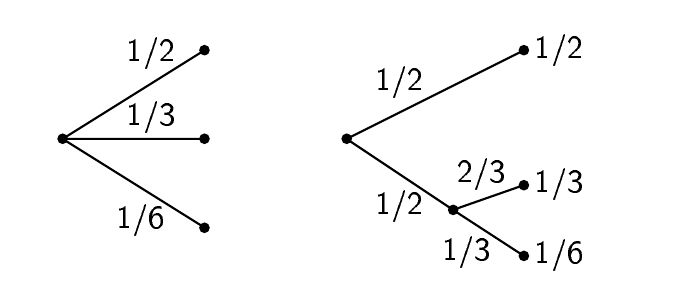
\includegraphics[scale=0.3]{Third_property.png}
            \captionof*{Figure}{In this particular case we require that
            $H(\frac{1}{2}, \frac{1}{3}, \frac{1}{6}) = 
            H(\frac{1}{2}, \frac{1}{2}) + \frac{1}{2} H(\frac{2}{3}, \frac{1}{3})$}
        \end{enumerate}
    \end{definition}

\end{frame}

\begin{frame}{Entropy cnt.}
    From the restrictions above, Shannon concluded that the only function,
    which satisfies all of the properties is the following:
    
    \begin{equation}
        H(\chi) = -\sum_{x \in \chi}{p(x) \log p(x) = \mathbb{E}(- \log p(\chi))}
    \end{equation}
    where $p(x)$ is the probability of event $x$.

\end{frame}

% https://en.wikipedia.org/wiki/Shannon%27s_source_coding_theorem
\begin{frame}{Basics of information theory}
    \section{Basics of information theory}
    \begin{theorem}[Source coding theorem]
    $N$ independed and identically distributed variables each with random 
    variables each with entropy $H(X)$ can be compressed into more than $NH(X)$ 
    bits with negligible risk of information loss, as $N \to \infty$; but 
    conversely, if they are compressed into fewer than $NH(X)$ bits it is 
    virtually certain that information will be lost.
    \end{theorem}
\end{frame}

\begin{frame}{Formal definition of PKC}
    \section{Formal definition of Public Key Cryptography}
    Public Key Cryptography consists of the public key, private key, 
    the encryption algorithm and the decryption algorithm. Let us see how these 
    things interact with each other.
\end{frame}

\begin{frame}{Formal definition of PKC}
    \begin{definition}[Public Key Cryptography\cite{galbraith_2012}]
        Let $\kappa$ be the security parameter of the cryptosystem. (note that 
        $\kappa$ is not necessarily the key length) An encryption scheme is then 
        defined by the following spaces (all depending on the security parameter 
        $\kappa$):
        \begin{itemize}
            \item $M_\kappa$ --- Space of all possible messages
            \item $PK_\kappa$ --- Space of all public keys
            \item $SK_\kappa$ --- Space of all secret keys
            \item $C_\kappa$ --- Space of all ciphertexts
            \item $KeyGen$ --- \textbf{Randomized} algorithm that takes $\kappa$ as input and generates
            public and private key in polynomial time. 
            \item $Encrypt : M_\kappa \times PK_\kappa \to C_\kappa$ 
            \item $Decrypt : C_\kappa \times SK_\kappa \to M_\kappa$
        \end{itemize}
    \end{definition}
\end{frame}

\begin{frame}{Constraint on $Encrypt$ and $Decrypt$}
    So, what is the most reasonable constraint that we can propose for the 
    $Encrypt$ and $Decrypt$ algorithms?
    \pause
    \begin{flalign*}
        & m \in M_\kappa, pk \in PK_\kappa, sk \in SK_\kappa \\ 
        & Decrypt(Encrypt(m, pk), sk) = m
    \end{flalign*}
\end{frame}

\begin{frame}{Trapdoor function}
    \section{Trapdoor function}
    \begin{definition}[Trapdoor function]
        The trapdoor function is such function that is easy to compute in one 
        way, but very hard (infeasible) to compute in other way in reasonable
        amount of time, computing resourses and manpower.
    \end{definition}

    \begin{example}
        \begin{itemize}
            \item Discrete Logarithm Problem (DLP) modulo $p$, where $p$ is large prime
            \item As generalization, DLP in large finite fields, where it is hard 
            to solve the DLP
            \item Shortest Vector Problem --- way to find the shortest vector 
            in the lattice
            \item Integer factorisation problem
            \item Syndrome decoding problem 
            \item Knapsack problem 
            \item etc.
        \end{itemize}    
    \end{example}
\end{frame}

\begin{frame}{Cryptographic primitives}
    \section{Cryptographic primitives}
    \begin{definition}
        Cryptographic primitive are well known cryptographic algorithms which 
        are used to build (cryptographic) protocols, e.g. 
        \begin{itemize}
            \item One way hash function
            \item Digital signature scheme 
            \item Symmetric key cryptography
            \item Public key cryptography
            \item etc.
        \end{itemize}
    \end{definition}
\end{frame}

\begin{frame}{Classification of cryptographic primitives}
    \subsection{Classification}
    As it was described in \cite{gagliardoni2017quantum}, one can divide 
    cryptographic primitives in the following categories:
    \begin{enumerate}
        \item QS0: Classical Security
        \item QS1: Post-Quantum Security
        \item QS2: Quantum (Superposition-Based) Security
        \item QS3: Fully Quantum Security
    \end{enumerate}
    We are interested only in the first two categories.
\end{frame}

\begin{frame}{How can we use cryptographic primitives?}
    \section{Usage of cryptographic primitives}
    \begin{example}
        As I mentioned earlier, in~\cite{diffie-hellman:1976} Diffie and Hellman
        proposed new key exchange protocol, we will dive deep into Diffie-Hellman 
        Key Exchange in lecture 5 (I hope).
    \end{example}
\end{frame}

\begin{frame}
    Its Jupyter Notebook time!
\end{frame}

\begin{frame}[allowframebreaks]{References}
	\section*{References}
	\bibliography{refs}
	\bibliographystyle{ieeetr}
\end{frame}

\end{document}
